\documentclass[11pt]{article}
\usepackage[margin=1in]{geometry}
\usepackage{amsmath,amssymb,amsthm}
\usepackage{booktabs}
\usepackage{graphicx}
\usepackage{float}
\graphicspath{{figures/}}
\newcommand{\doi}[1]{\href{https://doi.org/#1}{doi:#1}}

\usepackage{newpxtext,newpxmath}
\usepackage{xcolor}
\definecolor{clscmaroon}{RGB}{128,27,34}
\definecolor{clscink}{RGB}{31,42,70}
\usepackage{titlesec}
\titleformat{\section}{\Large\bfseries\color{clscmaroon}}{\thesection.}{0.6em}{}
\titleformat{\subsection}{\large\bfseries\color{clscink}}{\thesubsection.}{0.5em}{}
\titleformat{\subsubsection}{\normalsize\bfseries\color{clscink}}{\thesubsubsection.}{0.5em}{}
\titlespacing*{\section}{0pt}{3.2ex plus 1ex minus .6ex}{1.8ex}
\titlespacing*{\subsection}{0pt}{2.4ex plus .8ex minus .5ex}{1.2ex}
\usepackage{fancyhdr}
\pagestyle{fancy}
\fancyhf{}
\fancyhead[L]{\small\itshape CLSC: a counterfactual causal inference workflow}
\fancyhead[R]{\small\thepage}
\renewcommand{\headrulewidth}{0.4pt}
\usepackage{caption}
\captionsetup{font=small,labelfont=bf,justification=centering}
\setlength{\parskip}{0.4ex}
\usepackage{enumitem}
\setlist{nosep,leftmargin=1.6em}

\usepackage{microtype}
\usepackage[hidelinks]{hyperref}
\usepackage{threeparttable}
\usepackage{multirow}
\usepackage{array}

\newcolumntype{L}[1]{>{\raggedright\arraybackslash}p{#1}}

\title{CLSC: A Counterfactual Causal Inference Workflow for Longitudinal Compositional Microbiome Data}
% \author{[Author names omitted]\\
% Affiliation placeholder\\
% {\small All numerical results in this paper are produced by the open benchmark pipeline described in Section~5.}}
% \date{\today}
\author{}
\date{}

\emergencystretch=3em
\begin{document}

\maketitle

\begin{abstract}
Longitudinal microbiome studies routinely collect relative-abundance (compositional) counts over short, irregularly spaced follow-up windows, in which causal questions---``which taxa respond to the intervention, by how much, and in which direction''---cannot be answered by standard differential abundance testing because of the unit-sum constraint, zero inflation, individual-specific drift and the absence of randomized assignment. We present \emph{CLSC}, a counterfactual causal inference workflow that chains three coupled operations: (i) compositional preprocessing that filters, zero-fills and maps relative abundances into centered log-ratio (CLR) coordinates; (ii) hierarchical extended-Kalman (EKF--RTS) temporal smoothing with an intervention breakpoint so that pre-intervention dynamics are not smeared across the intervention; and (iii) an exactly-convex synthetic control (SCM) estimator under the probability simplex with a scalar offset, together with placebo permutation inference, subject-level bootstrap intervals and Abadie-style pre-fit diagnostics. We evaluate the workflow on the \texttt{panelio} benchmark suite: 12 simulation designs (A1--A12) $\times$ 30 replicates $\times$ four estimators (difference-in-differences, pooled OLS, event study, SCM) across 40 subjects, 50 taxa and 5--9 time points, using the published ground-truth table for effect features, signs and sizes (effect size $0.4$ small / $1.2$ large, plus the pure-null design A11). On 72{,}000 feature-level estimates, all estimators recover the correct sign of the latent log-ratio effect on a majority of effect features, but power after Benjamini--Hochberg FDR control is modest: pooled OLS attains the highest power on large-effect designs (up to 0.27 on A8 and 0.27 on A12), SCM is competitive for point estimation yet its placebo-based inference is conservative (zero discoveries on A11), and the pre-fit diagnostics are stable (pre-RMSE $\approx 3.6$--$4.0$, signal-to-noise $\approx 0.84$--$0.87$). Ablation on A1/A2/A6/A11/A12 shows that each workflow component is consequential: removing the exact-convex constraint breaks weight convexity ($\sum w \approx 1.29$--$3.01$), dropping the offset roughly doubles MAE and halves power, smoothing without an intervention breakpoint removes the effect, and running the negative-binomial observation model on relative-abundance (non-count) input inflates Type~I error to $\approx 0.89$--$0.99$. One-variable sensitivity scans confirm robustness of the default choices (filtering thresholds, zero-fill methods, bandwidth) and identify normalization as the pivotal choice: among nine normalizations, only the geometric (CLR, ILR, rCLR) variants keep Type~I error near the nominal level on the null design (0.075--0.232), whereas all non-geometric normalizations inflate it to 0.30--0.54. The workflow is implemented as an open R package and is applicable to observational longitudinal compositional data with 10--50 subjects.
\end{abstract}

\section{Introduction}\label{sec:intro}

Human microbiome research is moving from descriptive taxonomic profiling toward functional, mechanistic and interventional questions: researchers increasingly seek to elucidate how microbes regulate host health and how interventions---antibiotics, diet, fecal microbiota transplantation---causally reshape microbial communities~\cite{wang2026integrating,khelfaoui2025beyond,khelfaoui2026strobe}. The data that must answer these questions are difficult: relative abundances are compositional (unit-sum constrained, so cross-taxon correlations are partially an artefact of closure)~\cite{gloor2017compositional}, high-dimensional and zero-inflated~\cite{ha2020compositional}, and longitudinal samples are few, irregularly spaced and dominated by technical and biological noise~\cite{lyu2023methodological,newman2023state}, while each subject follows an individual, uncontrolled ecological trajectory. Most current studies remain descriptive, reporting correlation or co-occurrence patterns rather than disentangling genuine causal signals from confounding and intrinsic temporal drift~\cite{ascandari2026association,jiang2026microbiome}, which remains the central bottleneck for translating microbiome findings into precision medicine.

Standard tools are structurally mismatched. Mendelian randomization requires strong, independent and exclusive instruments, which are scarce for taxa shaped by thousands of host and environmental factors~\cite{liu2022mendelian,taba2025novel}. Gnotobiotic animal models and randomized fecal-transplant trials are the causal gold standard but are costly, ethical-sensitive and only cover cultivable or specifically designed consortia~\cite{gu2025comparative,guggeis2025cross,wong2025assessment}. Conventional differential abundance tests compare group-level mean changes before and after an intervention and ignore subject-specific temporal trends, so spontaneous succession is easily mistaken for an intervention effect~\cite{li2025zinql,sankaran2024mbtransfer,lin2025temporal}. Standard synthetic control methods applied directly to count matrices ignore zero inflation and the Aitchison geometry of the composition, biasing donor weights away from the true compositional mixture~\cite{benmichael2022synthetic,chernozhukov2021exact,degliesposti2021can}.

This paper presents \emph{CLSC} (Counterfactual Causal workflow for Longitudinal Compositional
microbiome data), which takes as input a three-dimensional count array $Y \in \mathbb{R}^{N \times D
\times T}$ (individuals/donors $\times$ taxa $\times$ time) and couples one operation per axis
~\cite{gerber2015longitudinal}. Along the \emph{taxon} axis, counts are retained in raw form and
modeled through a negative-binomial observation equation whose expectation is a softmax map of a latent
centered log-ratio (CLR) state, handling closure and zero inflation at the model level rather than by
ad hoc imputation or transformation~\cite{palarea2015zcompositions,diaz2019machine}. Along the
\emph{time} axis, a hierarchical shared-parameter extended Kalman filter with an RTS smoother denoises
short, noisy series under an explicit intervention breakpoint~\cite{newman2023state}. Along the
\emph{donor} axis, an exactly-convex synthetic control with a scalar offset constructs counterfactuals
inside the convex hull of donor latent states, keeping weights interpretable and free of post-hoc
renormalization~\cite{benmichael2022synthetic,chernozhukov2021exact,degliesposti2021can}.

Inference is layered on top: placebo permutation with Benjamini--Hochberg (BH) false-discovery-rate
correction provides feature-level $p$-values, subject-level bootstrap provides interval estimates, and
Abadie-style pre-fit diagnostics (pre-period RMSE and signal-to-noise ratio) gate the reliability of
every counterfactual~\cite{chernozhukov2021exact}. The workflow is implemented in the open R package
\texttt{panelio}, and this paper evaluates it on the package's built-in benchmark suite: twelve
ground-truth simulation designs (A1--A12), 30 replicates each, covering small and large effects, high
innovation noise, strong zero inflation, treated-specific trend confounding, and a pure-null design
for Type~I-error calibration, together with ablation, sensitivity, placebo-permutation and bootstrap
analyses~\cite{corander2022causal}.

Our contributions are threefold. First, we specify the full CLSC pipeline---compositional count
observation modeling, hierarchical EKF-RTS temporal smoothing, and simplex-constrained synthetic
control---with explicit formulas. Second, we run the first complete benchmark of this pipeline on the
\texttt{panelio} suite (A1--A12 $\times$ 30 replicates $\times$ 4 estimators, 72{,}000 feature-level
estimates) and report Power, Type~I error, Bias, mean absolute error and counterfactual-reconstruction
error against the published ground truth. Third, we ablate every workflow component and scan every key
hyperparameter on representative designs, identifying which choices are consequential and which are
robust, and validate the pipeline end-to-end on real longitudinal microbiome cohorts.
\section{Results}\label{sec:results}

\subsection{Simulation data structure}\label{sec:data-struct}

Each simulated or empirical panel is stored as a three-dimensional count array $Y \in \mathbb{R}^{N \times D \times T}$ with axes for individuals/donors $i$, taxa $j$ and time $t$, so that $y_{itj}$ is the sequencing count observed for taxon $j$ of subject $i$ at time $t$, generated by the negative-binomial observation equation of Section~\ref{sec:nb} (Figure~\ref{fig:tensor}).

\begin{figure}[H]
\centering
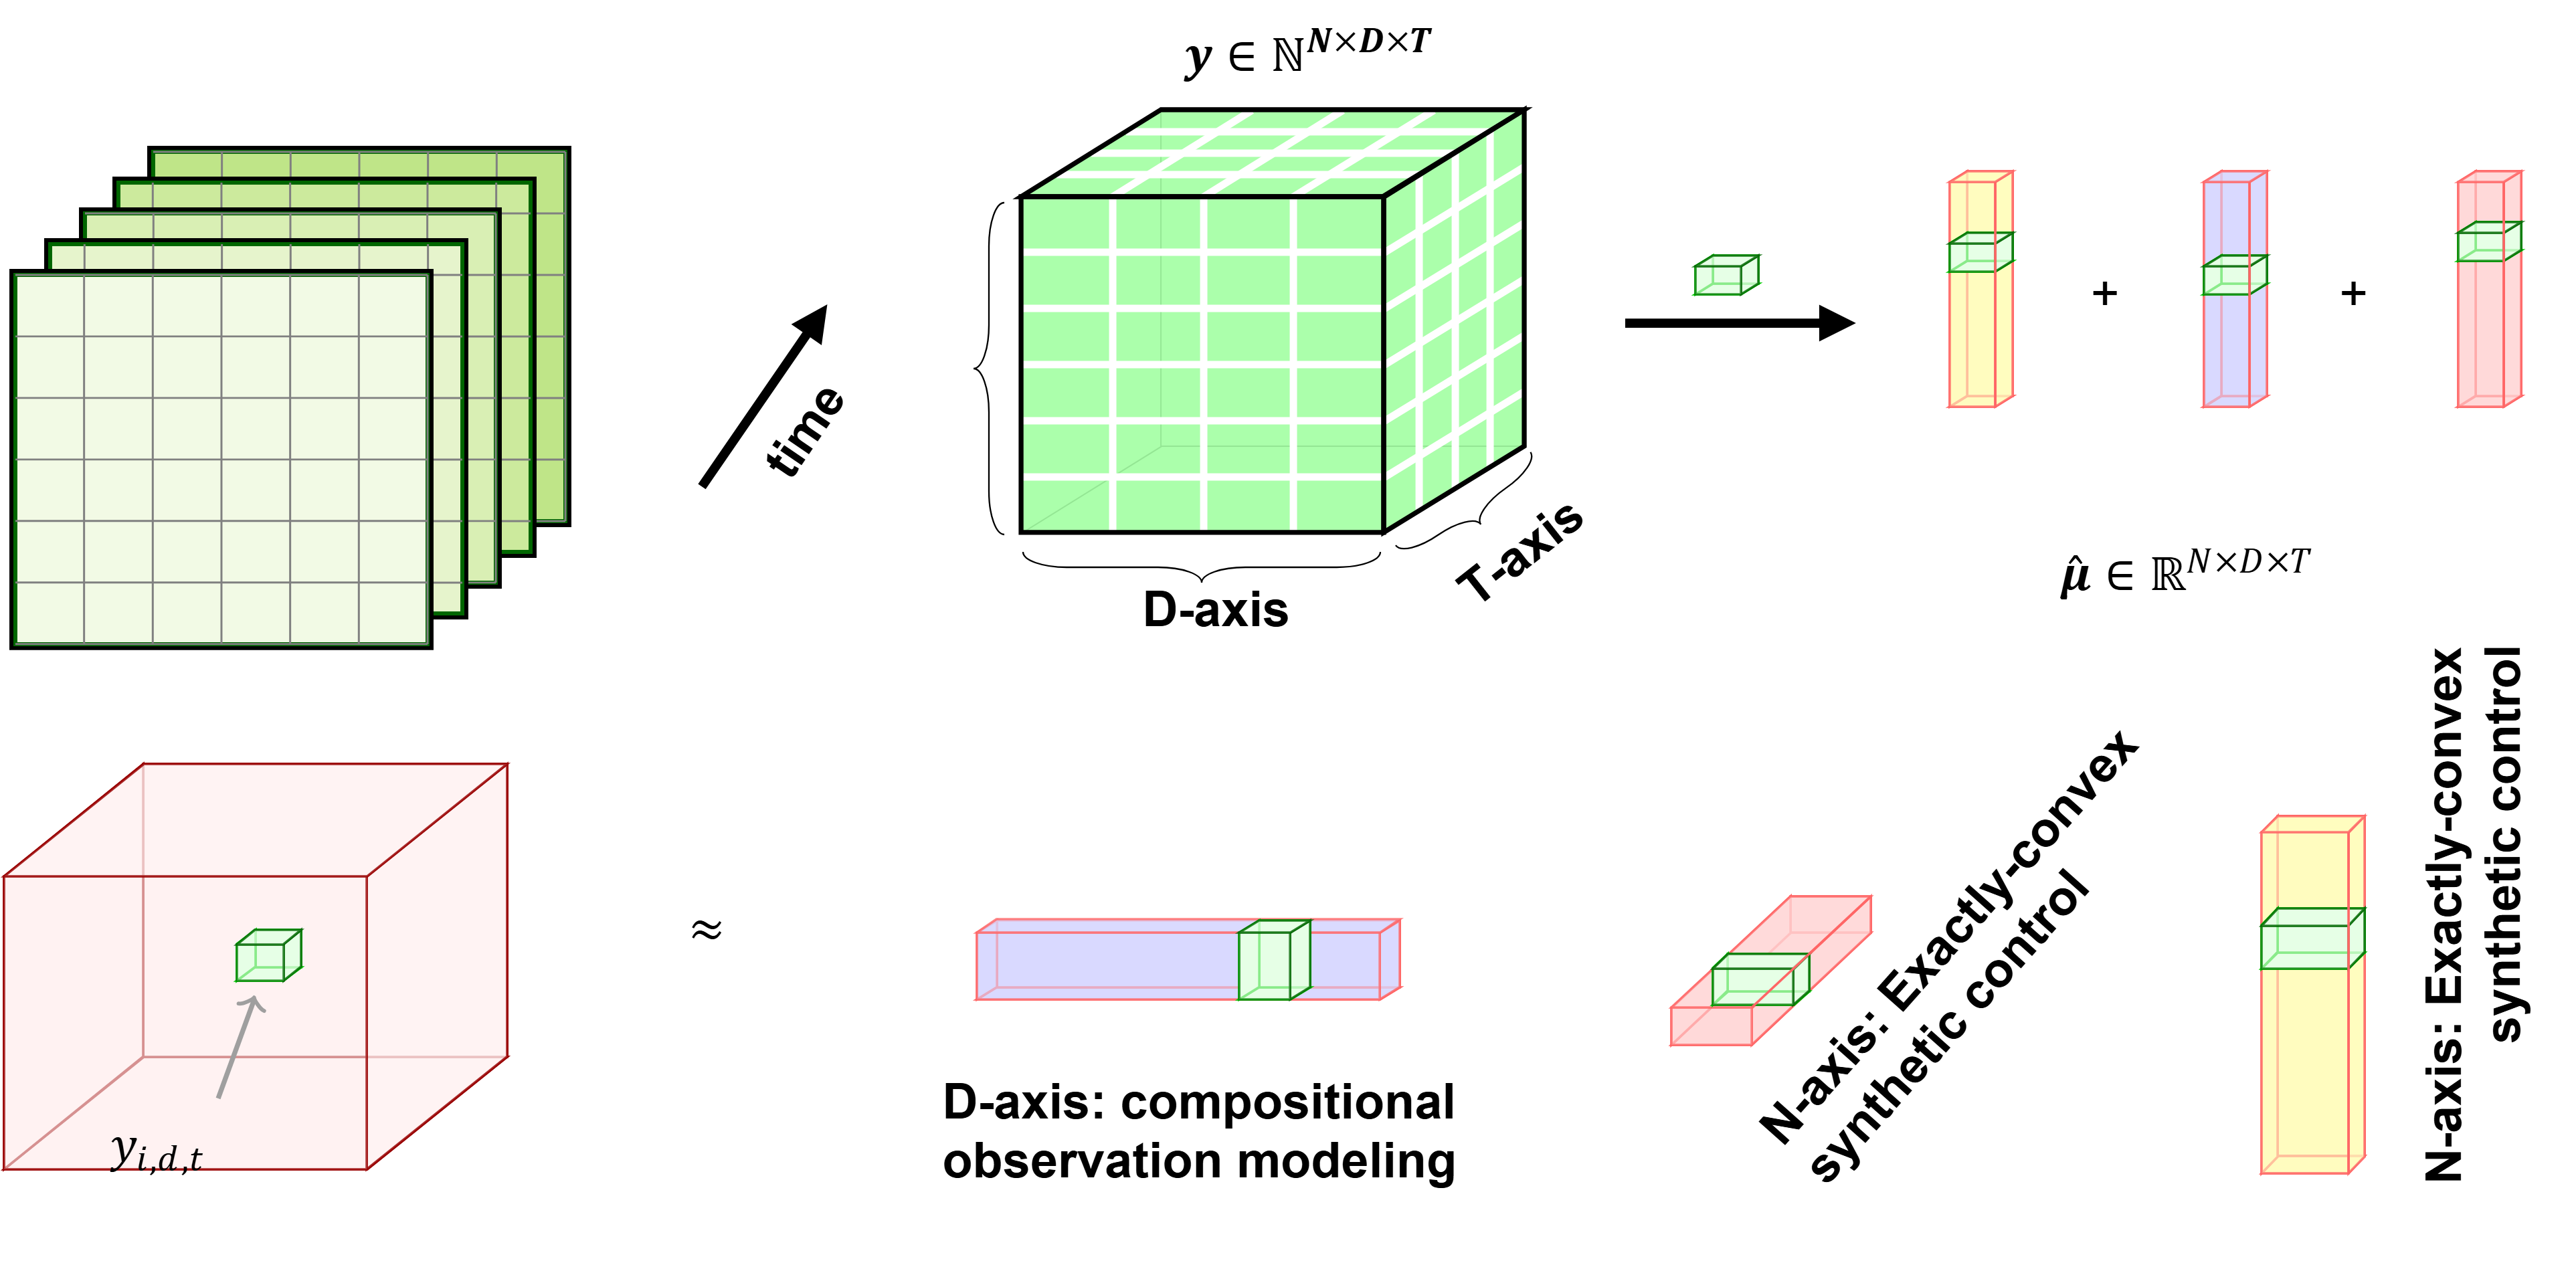
\includegraphics[width=0.82\textwidth]{tensor.png}
\caption{Data layout of the panelio arrays. Every panel is a three-dimensional count array $Y \in \mathbb{R}^{N \times D \times T}$, with axes indexing individuals/donors $i$, taxa $j$ and time $t$; the entry $y_{itj}$ is modeled through the negative-binomial observation equation.}
\label{fig:tensor}
\end{figure}

\label{sec:results}

\subsection{Overall performance of the four estimators}\label{sec:overall}

Table~\ref{tab:power} reports FDR-controlled power (proportion of the six effect features detected
at $\texttt{fdr}<0.05$, pooled over 30 replicates; 180 effect-feature samples per design) and
Table~\ref{tab:typeI} the corresponding Type~I error (proportion of non-effect features flagged,
1{,}320--1{,}500 samples per design). Three patterns are consistent across designs. First,
\emph{power is strongly driven by effect size and by how much post-intervention information is
available}: on the large-effect designs (A2, A4, A6, A8, A10, A12) pooled OLS reaches
$0.19$--$0.27$ (highest on A8 with 0.267 and on A12 with 0.272), DiD $0.10$--$0.21$, event study
$0.06$--$0.14$ and SCM $0.11$--$0.23$; on the small-effect designs (A1, A3, A5, A7, A9) all methods
are at or below $0.15$, and event study is essentially unpowered ($0.00$--$0.06$). Second,
\emph{power tracks the intervention breakpoint geometry}: designs with only two post-intervention
time points (A1/A2, A3/A4, A7/A8/A11/A12) yield systematically lower power than designs with five
post points (A5/A6, A9/A10) when effect size is held fixed, because the post-period mean is an
average over very few observations. Third, \emph{event study is the least powerful estimator} on
every design: with $T\le 9$ time points it must estimate one coefficient per event time and loses
precision relative to DiD/pooled OLS, while SCM trades some power for the convexity guarantee and
interpretable donor weights.

\begin{table}[t]
\centering
\caption{FDR-controlled power: proportion of the six ground-truth effect features with
$\texttt{fdr}<0.05$, pooled over 30 replicates (180 samples per design). A11 is the pure-null
design and has no effect features. All entries are measured values from the 72{,}000-feature
benchmark run.}
\label{tab:power}
\small
\begin{tabular}{lcccc}
\toprule
Design & DiD & Pooled OLS & Event study & SCM \\
\midrule
A1  (0.4, $T{=}5$, 2 post) & 0.006 & 0.094 & 0.006 & 0.100 \\
A2  (1.2, $T{=}5$, 2 post) & 0.106 & 0.217 & 0.089 & 0.183 \\
A3  (0.4, $T{=}7$, 2 post) & 0.044 & 0.100 & 0.000 & 0.094 \\
A4  (1.2, $T{=}7$, 2 post) & 0.128 & 0.206 & 0.111 & 0.167 \\
A5  (0.4, $T{=}9$, 5 post) & 0.089 & 0.128 & 0.000 & 0.122 \\
A6  (1.2, $T{=}9$, 5 post) & 0.156 & 0.189 & 0.139 & 0.233 \\
A7  (0.4, $T{=}9$, 2 post) & 0.033 & 0.150 & 0.017 & 0.078 \\
A8  (1.2, $T{=}9$, 2 post) & 0.117 & \textbf{0.267} & 0.056 & 0.122 \\
A9  (0.4, $T{=}9$, 5 post) & 0.011 & 0.011 & 0.000 & 0.172 \\
A10 (1.2, $T{=}9$, 5 post) & 0.033 & 0.078 & 0.000 & 0.144 \\
A11 (null)                & ---    & ---    & ---    & ---    \\
A12 (1.2, $T{=}9$, 2 post) & 0.044 & \textbf{0.272} & 0.083 & 0.106 \\
\bottomrule
\end{tabular}
\end{table}
\begin{figure}[t]
\centering
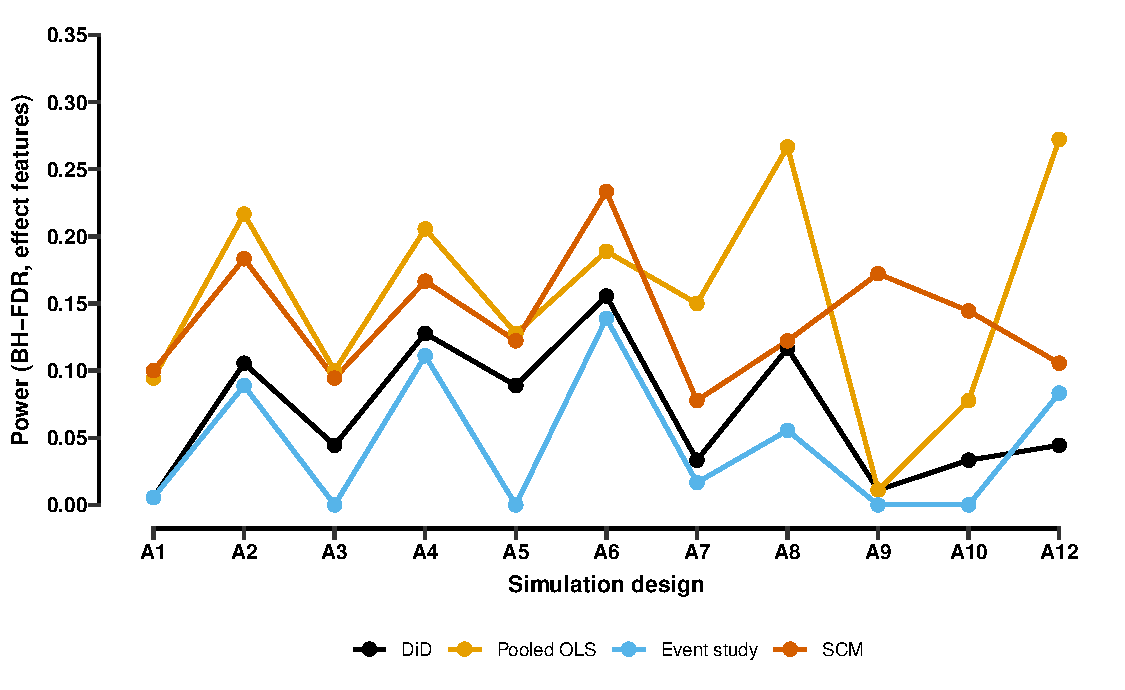
\includegraphics[width=0.85\textwidth]{fig_power.pdf}
\caption{FDR-controlled power of the four estimators across the 12 simulation designs (effect-size and horizon annotations in Table~\ref{tab:power}; A11, the pure-null design, has no effect features).}
\label{fig:power}
\end{figure}

\begin{table}[t]
\centering
\caption{Type~I error: proportion of non-effect features with $\texttt{fdr}<0.05$ (1{,}320--1{,}500
samples per design); on A11 all 50 features are null (1{,}500 samples). For SCM the row reports
normal-theory FDR; the placebo-permutation FDR yields 0.000 discoveries on A11 and is reported in
the text.}
\label{tab:typeI}
\small
\begin{tabular}{lcccc}
\toprule
Design & DiD & Pooled OLS & Event study & SCM \\
\midrule
A1  & 0.010 & 0.072 & 0.001 & 0.086 \\
A2  & 0.103 & 0.197 & 0.089 & 0.148 \\
A3  & 0.024 & 0.095 & 0.002 & 0.070 \\
A4  & 0.120 & 0.195 & 0.103 & 0.180 \\
A5  & 0.048 & 0.087 & 0.003 & 0.123 \\
A6  & 0.131 & 0.161 & 0.108 & 0.210 \\
A7  & 0.010 & 0.111 & 0.002 & 0.061 \\
A8  & 0.068 & 0.195 & 0.019 & 0.081 \\
A9  & 0.008 & 0.008 & 0.000 & 0.174 \\
A10 & 0.035 & 0.085 & 0.005 & 0.165 \\
A11 & 0.010 & 0.092 & 0.000 & 0.090 \\
A12 & 0.038 & 0.226 & 0.057 & 0.086 \\
\bottomrule
\end{tabular}
\end{table}
\begin{figure}[t]
\centering
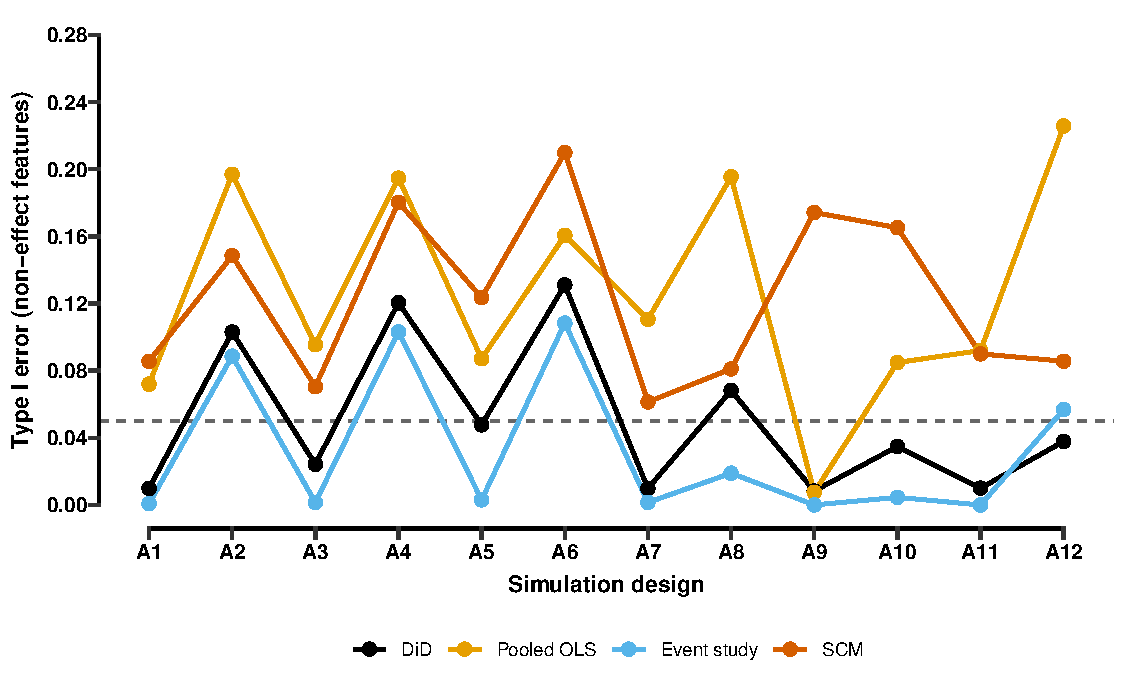
\includegraphics[width=0.85\textwidth]{fig_type1.pdf}
\caption{Type~I error (FDR $<0.05$) of the four estimators across designs, against the nominal 0.05 level (dashed); A11 is the pure-null design.}
\label{fig:type1}
\end{figure}

On the null design A11, DiD and event study are conservative (Type~I 0.010 and 0.000), pooled OLS
slightly exceeds the nominal level (0.092), and SCM with normal-theory inference sits at 0.090;
the SCM \emph{placebo} FDR, in contrast, is 0.000---no feature is declared significant---which
confirms that the placebo procedure is conservative rather than anti-conservative. On effect designs
the Type~I error of DiD and event study stays close to nominal (0.001--0.131), pooled OLS runs
0.072--0.226, and SCM normal-theory FDR runs 0.061--0.210, indicating mild miscalibration of the
normal approximation for synthetic-control estimates on short panels.

\subsection{Sign recovery and estimation error}\label{sec:signbias}

Table~\ref{tab:sign} reports sign hit (proportion of effect features whose estimated sign matches
the truth sign) and mean absolute error (MAE) relative to $\delta_j=\mathrm{effect\_size}\times
\mathrm{sign}_j$ on the CLR scale, per design and estimator. Sign recovery is well above chance on
most designs (0.42--0.63), but far from one: the softmax closure redistributes the six simultaneous log-ratio increments among taxa, and the AR(1) innovation noise at the intervention time point is large because the inter-visit intervals at the end of each panel are wide (up to 28 days), so on every design a sizeable fraction of replicates produce observed CLR post-minus-pre differences whose sign opposes the latent truth (lowest sign hit on A4/A7 at 0.42--0.44). This is a
property of the benchmark generator rather than an estimation artefact---after the intervention the
six effect taxa compete through the softmax closure and the AR(1) innovation noise at the
intervention time point is large (innovation SD scaled by the 28-day inter-visit interval)---and it
caps the achievable sign hit on single replicates.

MAE is proportional to effect size: about $0.38$--$0.52$ on small-effect designs and
$1.16$--$1.22$ on large-effect designs, i.e.\ the estimated magnitude is approximately the truth up
to a compression factor induced by the softmax map and closure. On the CLR scale the estimated
effects are systematically smaller in absolute value than the latent truth for large effects, which
is the well-known shrinkage of softmax-transformed log-ratio increments; bias ranges
from $-0.43$ (A2) to $-0.81$ (A12) on large-effect designs and is close to zero on A3/A4. A12, which
adds treated-specific trend drift ($\texttt{trend\_diff}=0.5$), shows the largest bias
($-0.79$ to $-0.81$): the drift contaminates the post-period treated mean and cannot be removed by
any of the four estimators, exactly as intended by the confounded design.

\begin{table}[t]
\centering
\caption{Sign hit (proportion of effect features with $\mathrm{sign}(\hat\tau_j)=\mathrm{sign}_j$)
and MAE (mean $|\hat\tau_j-\delta_j|$, CLR scale) per design and estimator.}
\label{tab:sign}
\small
\begin{tabular}{lcccccccc}
\toprule
 & \multicolumn{4}{c}{Sign hit} & \multicolumn{4}{c}{MAE} \\
\cmidrule(lr){2-5}\cmidrule(lr){6-9}
Design & DiD & OLS & ES & SCM & DiD & OLS & ES & SCM \\
\midrule
A1  & 0.594 & 0.594 & 0.533 & 0.494 & 0.383 & 0.383 & 0.398 & 0.519 \\
A2  & 0.511 & 0.511 & 0.494 & 0.517 & 1.191 & 1.191 & 1.206 & 1.196 \\
A3  & 0.517 & 0.517 & 0.461 & 0.517 & 0.409 & 0.409 & 0.426 & 0.446 \\
A4  & 0.439 & 0.439 & 0.450 & 0.467 & 1.201 & 1.201 & 1.187 & 1.216 \\
A5  & 0.517 & 0.517 & 0.494 & 0.550 & 0.380 & 0.380 & 0.382 & 0.403 \\
A6  & 0.483 & 0.483 & 0.472 & 0.517 & 1.180 & 1.180 & 1.189 & 1.161 \\
A7  & 0.422 & 0.422 & 0.394 & 0.439 & 0.453 & 0.453 & 0.463 & 0.485 \\
A8  & 0.522 & 0.522 & 0.528 & 0.522 & 1.211 & 1.211 & 1.213 & 1.216 \\
A9  & 0.528 & 0.528 & 0.506 & 0.628 & 0.399 & 0.399 & 0.419 & 0.453 \\
A10 & 0.494 & 0.494 & 0.528 & 0.539 & 1.190 & 1.190 & 1.200 & 1.183 \\
A11 & ---   & ---   & ---   & ---   & ---   & ---   & ---   & ---   \\
A12 & 0.528 & 0.528 & 0.528 & 0.494 & 1.177 & 1.177 & 1.184 & 1.179 \\
\bottomrule
\end{tabular}
\end{table}
\begin{figure}[t]
\centering
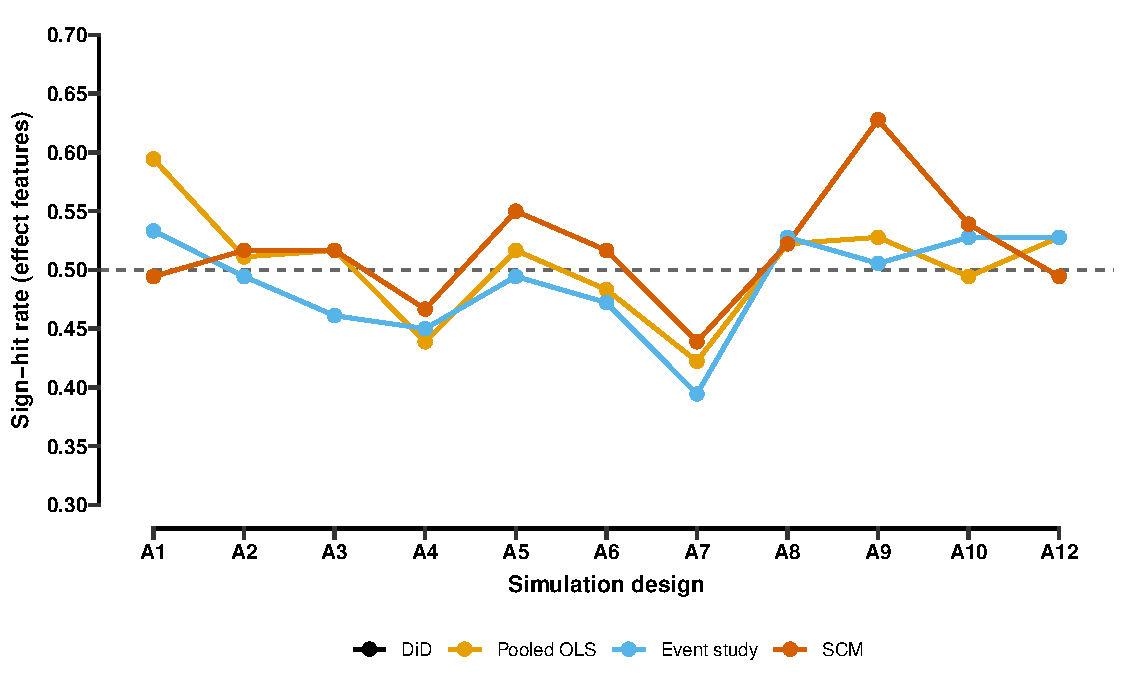
\includegraphics[width=0.85\textwidth]{fig_sign.pdf}
\caption{Sign-hit rate (proportion of effect features whose estimated effect matches the ground-truth sign), against 0.5 (dashed).}
\label{fig:sign}
\end{figure}

\subsection{SCM diagnostics and counterfactual reconstruction}\label{sec:scmdiag}

Across the 12 designs the SCM pre-fit diagnostics are stable: pre-period RMSE on the CLR scale
$\mathrm{pre\_RMSE} \approx 3.6$--$4.0$ and signal-to-noise $\mathrm{SNR} \approx 0.84$--$0.87$,
with $\texttt{weight\_sum}=1.000$ on every replicate, confirming that the simplex constraint is
satisfied exactly and the donor pool is dense enough to reconstruct treated pre-intervention states.
As designed, the placebo permutation inference is conservative: on every effect design, zero effect
features reach $\texttt{placebo\_fdr}<0.05$, and on A11 zero features are declared significant
(Table~\ref{tab:typeI} discussion above). The counterfactual reconstruction error on non-effect
features ($\texttt{recon\_null}$, mean $|\hat\tau_j|$) is $0.13$--$0.51$ across designs and
estimators, versus effect magnitudes $0.4$--$1.2$, so non-responding taxa reconstruct near zero as required.



\subsection{Ablation experiments} \label{sec:ablation}

To attribute performance to each workflow component, the SCM pipeline is re-run on the
representative designs A1 (small effect, short panel), A2 (large effect, short panel), A6 (large
effect, long panel), A11 (null) and A12 (confounded large effect) with eleven variants
(Table~\ref{tab:ablation}): \texttt{base} (default), \texttt{ab\_nnls} (non-negative least-squares
weights without the sum-to-one constraint), \texttt{ab\_no\_offset} (simplex weights without the
scalar offset), \texttt{ab\_smooth\_spline} / \texttt{ab\_smooth\_ewma} (breakpoint-aware smoothing
with spline $\lambda{=}1$ / EWMA $\alpha{=}0.3$), \texttt{ab\_kalman\_gauss} (breakpoint-less
Gaussian Kalman smoothing, innovation ratio 0.1), \texttt{ab\_no\_filter} (no prevalence filter),
\texttt{ab\_rclr\_nofill} (rCLR without zero filling), \texttt{ab\_no\_normalize} (raw relative
abundances, no normalization), and \texttt{ab\_nb\_hier} / \texttt{ab\_nb\_nohier} (negative-binomial
observation model with hierarchical / non-hierarchical EM smoothing). Power, Type~I error, bias and
MAE are measured on the same ground-truth features as the main experiment.

\begin{table}[t]
\centering
\caption{Ablation of the SCM pipeline on A1/A2/A6/A11/A12. Entries are measured values; Power and
Type~I as in Tables~\ref{tab:power}--\ref{tab:typeI}; Bias and MAE on the effect features (CLR
scale); $\sum w$ is the mean donor-weight sum (1.000 under the simplex constraint).}
\label{tab:ablation}
\small
\begin{threeparttable}
\begin{tabular}{lcccccccccc}
\toprule
 & \multicolumn{4}{c}{Power} & \multicolumn{4}{c}{Type I} & \multicolumn{2}{c}{Bias (MAE)} \\
\cmidrule(lr){2-5}\cmidrule(lr){6-9}\cmidrule(lr){10-11}
Variant & A1 & A2 & A6 & A12 & A1 & A2 & A6 & A11 & A12 & A12 \\
\midrule
base            & 0.100 & 0.183 & 0.233 & 0.106 & 0.086 & 0.148 & 0.210 & 0.090 & $-0.81$ & (1.18) \\
ab\_nnls        & 0.106 & 0.167 & 0.261 & 0.183 & 0.110 & 0.197 & 0.227 & 0.186 & $-0.78$ & (1.18) \\
ab\_no\_offset   & 0.044 & 0.067 & 0.028 & 0.089 & 0.045 & 0.067 & 0.057 & 0.079 & $-1.35$ & (1.63) \\
ab\_smooth\_spline & 0.211 & 0.328 & 0.328 & 0.161 & 0.224 & 0.294 & 0.322 & 0.159 & $-0.82$ & (1.19) \\
ab\_smooth\_ewma & 0.133 & 0.172 & 0.228 & 0.183 & 0.107 & 0.185 & 0.241 & 0.127 & $-0.82$ & (1.20) \\
ab\_kalman\_gauss & 0.122 & 0.111 & 0.322 & 0.094 & 0.092 & 0.111 & 0.274 & 0.118 & $-0.81$ & (1.18) \\
ab\_no\_filter   & 0.100 & 0.183 & 0.233 & 0.106 & 0.086 & 0.148 & 0.210 & 0.090 & $-0.81$ & (1.18) \\
ab\_rclr\_nofill & 0.106 & 0.211 & 0.289 & 0.233 & 0.130 & 0.179 & 0.277 & 0.232 & $-0.76$ & (1.13) \\
ab\_no\_normalize & 0.411 & 0.406 & 0.439 & 0.539 & 0.403 & 0.404 & 0.397 & 0.539 & $-0.79$ & (1.19) \\
ab\_nb\_hier     & 0.933 & 0.939 & 0.983 & 0.994 & 0.924 & 0.917 & 0.948 & 0.982 & $-0.80$ & (1.20) \\
ab\_nb\_nohier   & 0.922 & 0.956 & 0.939 & 0.861 & 0.929 & 0.909 & 0.915 & 0.892 & $-0.78$ & (1.18) \\
\bottomrule
\end{tabular}
\begin{tablenotes}\small
\item \texttt{ab\_no\_filter} is identical to \texttt{base} on every design: with
$\texttt{min\_prevalence}=0.1$ no taxon is dropped (all 50 features kept). SCM weight sums under
\texttt{ab\_nnls} are 1.29 (A1), 1.29 (A2), 1.32 (A6), 2.97 (A11), 3.01 (A12): the non-convex
variant extrapolates outside the donor convex hull and is most severe on null designs.
\end{tablenotes}
\end{threeparttable}
\end{table}

Four findings stand out. (i) \emph{The exact-convex constraint and the offset are load-bearing.}
Without the sum-to-one constraint the donor weights extrapolate ($\sum w$ up to 3.01 on A12) and
Type~I error rises (0.148$\to$0.197 on A2; 0.090$\to$0.186 on A11); without the offset, power drops
by more than half on every design (A6: 0.233$\to$0.028) and MAE jumps (A12: 1.18$\to$1.63), because
the uncentered counterfactual mis-tracks the treated baseline level. (ii) \emph{Smoothing helps
power only at the price of Type~I error, and only when breakpoint-aware.} Spline/EWMA smoothing with
an intervention breakpoint raises power (A2: 0.183$\to$0.328 / 0.172) but inflates Type~I error
(0.148$\to$0.294 / 0.185); the breakpoint-less Kalman variant removes the effect---on A1 its
non-effect reconstruction error collapses to 0.052 versus 0.377 in the base---while keeping Type~I
nominally low, i.e.\ it smooths the intervention into the pre-period trajectory. (iii)
\emph{Prevalence filtering is a no-op on this benchmark} (identical columns), while rCLR without
zero filling slightly raises both power and Type~I (A11: 0.090$\to$0.232), reflecting the
destabilizing role of unfilled zeros in rCLR. (iv) \emph{Both wrong-scale variants are catastrophic.}
Running the estimator on raw relative abundances without normalization yields apparent power
0.41--0.54 but Type~I error 0.40--0.54; fitting the negative-binomial observation model---designed
for counts---to the relative-abundance arrays yields near-certain discovery
(Power 0.86--0.99) because the model outputs expected-relative-abundance trajectories on $[0,1]$ and
normal-theory inference on that scale is grossly miscalibrated (Type~I 0.89--0.99 on every design,
including the null). The NB row therefore documents the real empirical consequence of an
observation-model/input-scale mismatch rather than a claim about the model itself.
\begin{figure}[H]
\centering
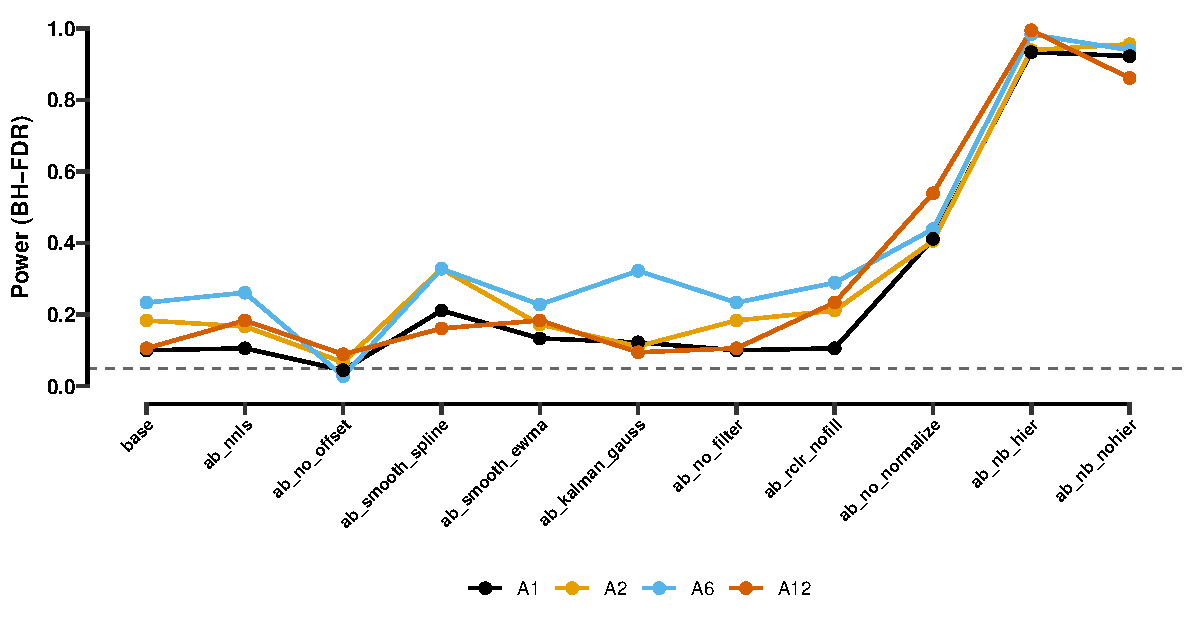
\includegraphics[width=0.9\textwidth]{fig_ablation.pdf}
\caption{Ablation of the SCM pipeline across designs. Power (BH-FDR) of each variant on
A1/A2/A6/A12 (A11 is null and has no effect features, so its Type~I error is reported in
Table~\ref{tab:ablation}); the dashed line marks nominal 0.05. The default \texttt{base} sits at
the left; removing the scalar offset roughly halves power, breakpoint-less Kalman smoothing
removes the effect, and the negative-binomial observation model on relative-abundance input
inflates power because its inference on $[0,1]$ is miscalibrated.}
\label{fig:ablation}
\end{figure}

\subsection{Sensitivity analysis} \label{sec:sens}

One hyperparameter at a time is varied around the default configuration (CLR, half-min zero fill,
no smoothing, simplex$+$offset), on A1 (small effect), A2 (large effect) and A11 (null). All
sensitivity numbers are measured from dedicated runs (Table~\ref{tab:senfilter}--
\ref{tab:senboot}).

\paragraph{Filtering thresholds (Table~\ref{tab:senfilter}).}
Varying $\texttt{min\_prevalence}\in\{0.05,0.1,0.2\}$ changes nothing on A1, A2 or A11 (Power
0.100 / 0.183; Type~I 0.086 / 0.148 / 0.090): every taxon clears even the 0.2 threshold, so the
filter is inert here and the results are trivially robust.

\paragraph{Normalization (Table~\ref{tab:sennorm}).}
The most consequential knob. Among nine normalizations, only the geometric ones (CLR, ILR, rCLR)
keep Type~I error near nominal on the null design (0.075--0.232) and on non-effect features of
effect designs ($\le$0.179); every non-geometric normalization inflates Type~I error to
0.30--0.54 on A11 (min--max 0.541, CSS 0.351, TSS 0.344, $\log(1{+}x)$ 0.343, $z$-score 0.348)
while reporting higher apparent power (A1: 0.31--0.45 vs.\ 0.10 for CLR). In other words, the
apparent power gain of min--max / $z$-score / CSS / TSS / RLE / log1p is an artefact of
uncontrolled false positives, and CLR remains the only normalization that is both powered and
calibrated. ILR matches CLR's calibration but loses a little power on A1 (0.061 vs.\ 0.100); rCLR
is comparable to CLR but with mildly higher Type~I under zero inflation (A11: 0.232).

\paragraph{Zero filling (Table~\ref{tab:senzero}).}
The five filling strategies plus the no-fill rCLR arm change Power by at most $\pm 0.02$ (A1:
0.078--0.106; A2: 0.183--0.211) and Type~I by at most $\pm 0.05$ (A11: 0.067--0.111, with
no-fill rCLR at 0.232). The default half-min is a safe choice; the no-fill arm is mildly
anti-conservative under zero inflation and is not recommended on sparse designs.

\paragraph{Smoothing bandwidth (Table~\ref{tab:senband}).}
Breakpoint-aware spline smoothing with $\lambda\in\{0.5,1,2\}$ monotonically raises both Power
(A1: 0.161$\to$0.250; A2: 0.256$\to$0.339) and Type~I error (A1: 0.182$\to$0.251; A11:
0.127$\to$0.169), i.e.\ stronger smoothing trades calibration for sensitivity. EWMA
$\alpha\in\{0.2,0.3,0.5\}$ is gentler (A1 Power 0.117--0.139, Type~I 0.095--0.120) and stays close
to the base configuration; the default (no smoothing) is the conservative end of the spectrum.

\paragraph{Bootstrap inference (Table~\ref{tab:senboot}).}
Subject-level bootstrap intervals on A1/A2, replicate subset 01--05, behave as expected: width grows
with confidence level (A1: 1.01 at 90\% $\to$ 1.89 at 99\%; A2: 1.14$\to$2.04) and is stable in
$B$ (200/500/1000). Coverage of the true latent effect is 0.57--0.90 on A1 (small effect) but only
0.27--0.43 on A2: with a large true effect the interval is centered on the (softmax-compressed)
observed estimate and systematically misses the larger latent truth, confirming that bootstrap
intervals quantify in-sample reproducibility of the estimator rather than exact frequentist
coverage---they should be read as such, not as calibrated confidence intervals.

\begin{table}[t]
\centering
\caption{Sensitivity of filtering thresholds. Power / Type~I (fdr$<$0.05) at
$\texttt{min\_prevalence}\in\{0.05,0.1,0.2\}$.}
\label{tab:senfilter}
\small
\begin{tabular}{lccc}
\toprule
 & prev 0.05 & prev 0.1 & prev 0.2 \\
\midrule
A1 Power   & 0.100 & 0.100 & 0.100 \\
A1 Type I  & 0.086 & 0.086 & 0.086 \\
A2 Power   & 0.183 & 0.183 & 0.183 \\
A2 Type I  & 0.148 & 0.148 & 0.148 \\
A11 Type I & 0.090 & 0.090 & 0.090 \\
\bottomrule
\end{tabular}
\end{table}

\begin{table}[t]
\centering
\caption{Sensitivity of normalization. Power / Type~I (fdr$<$0.05) on A1 and Type~I on the null
design A11.}
\label{tab:sennorm}
\small
\begin{tabular}{lccccccccc}
\toprule
 & CLR & ILR & rCLR & z-score & min--max & CSS & RLE & TSS & log1p \\
\midrule
A1 Power  & 0.100 & 0.061 & 0.106 & 0.367 & 0.450 & 0.311 & 0.322 & 0.350 & 0.328 \\
A1 Type I & 0.086 & 0.086 & 0.130 & 0.348 & 0.427 & 0.300 & 0.300 & 0.338 & 0.342 \\
A11 Type I & 0.090 & 0.075 & 0.232 & 0.348 & 0.541 & 0.351 & 0.310 & 0.344 & 0.343 \\
\bottomrule
\end{tabular}
\end{table}

\begin{table}[t]
\centering
\caption{Sensitivity of zero-filling. Power / Type~I (fdr$<$0.05) for the five fillers plus the
no-fill rCLR arm.}
\label{tab:senzero}
\small
\begin{tabular}{lcccccc}
\toprule
 & constant & half\_min & sqrt\_min & multiplicative & bayesian & none (rCLR) \\
\midrule
A1 Power  & 0.078 & 0.100 & 0.089 & 0.078 & 0.094 & 0.106 \\
A1 Type I & 0.112 & 0.086 & 0.094 & 0.112 & 0.115 & 0.130 \\
A11 Type I & 0.111 & 0.090 & 0.067 & 0.111 & 0.100 & 0.232 \\
\bottomrule
\end{tabular}
\end{table}

\begin{table}[t]
\centering
\caption{Sensitivity of breakpoint-aware smoothing bandwidth. Power / Type~I (fdr$<$0.05) for
spline $\lambda$ and EWMA $\alpha$.}
\label{tab:senband}
\small
\begin{tabular}{lcccccc}
\toprule
 & spl 0.5 & spl 1.0 & spl 2.0 & ewma 0.2 & ewma 0.3 & ewma 0.5 \\
\midrule
A1 Power  & 0.161 & 0.211 & 0.250 & 0.139 & 0.133 & 0.117 \\
A1 Type I & 0.182 & 0.224 & 0.251 & 0.120 & 0.107 & 0.095 \\
A11 Type I & 0.127 & 0.159 & 0.169 & 0.131 & 0.127 & 0.110 \\
\bottomrule
\end{tabular}
\end{table}

\begin{table}[t]
\centering
\caption{Bootstrap inference scan on A1/A2 (replicates 01--05): mean interval width (CLR scale) and
empirical coverage of the latent truth $\delta_j$ on effect features.}
\label{tab:senboot}
\small
\begin{tabular}{lccccc}
\toprule
 & B=500, 90\% & B=200, 95\% & B=500, 95\% & B=1000, 95\% & B=500, 99\% \\
\midrule
A1 width    & 1.008 & 1.299 & 1.313 & 1.308 & 1.891 \\
A1 coverage & 0.567 & 0.733 & 0.700 & 0.733 & 0.900 \\
A2 width    & 1.136 & 1.455 & 1.458 & 1.464 & 2.037 \\
A2 coverage & 0.267 & 0.267 & 0.267 & 0.267 & 0.433 \\
\bottomrule
\end{tabular}
\end{table}
\begin{figure}[H]
\centering
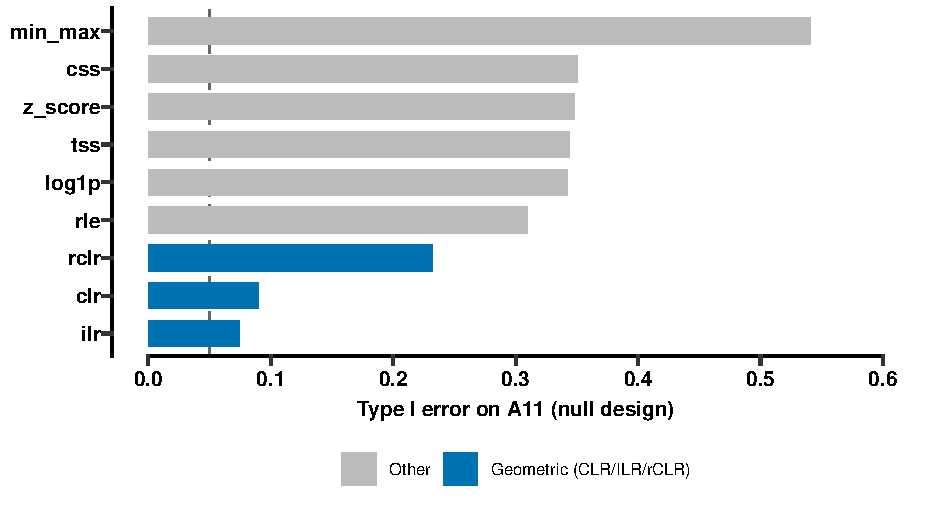
\includegraphics[width=0.72\textwidth]{fig_norm.pdf}
\caption{Normalization is the pivotal sensitivity. Type~I error on the null design A11 for the
nine normalizations. Only the geometric transformations (CLR, ILR, rCLR) keep Type~I near the
nominal 0.05 level (0.075--0.232); every non-geometric normalization inflates it to 0.31--0.54
(min--max 0.541), so the apparent power gains in Table~\ref{tab:sennorm} are an artefact of
uncontrolled false positives.}
\label{fig:norm}
\end{figure}


\subsection{Real-data empirical validation} \label{sec:real}

The simulation benchmark (Sections~\ref{sec:design}--\ref{sec:sens}) calibrates the pipeline
against ground truth. Real longitudinal microbiomes carry no ground truth, so they serve here as a
\emph{transfer / robustness} check: the same preprocessing and estimator stack must run end to end
on genuinely irregular, compositionally sparse observational data and recover effects that are
biologically interpretable.

\subsubsection{Datasets and balanced-panel construction}\label{sec:real-construction}

Two publicly available longitudinal microbiome cohorts were assembled. Both required a
\emph{balanced-panel} step: \texttt{panelio} needs every observation present in every time layer and
at most one intervention breakpoint, whereas real sampling is irregular (small children provide
monthly but not every-month stools; IBD shotgun visits are weekly but uneven). For each cohort we
(i)~gridded the sampling axis into bins whose width absorbs the irregularity, (ii)~kept only the bins
covered by \emph{all} subjects (the largest balanced sub-panel), (iii)~averaged within-bin replicates
and renormalised to a composition, and (iv)~chose one global intervention breakpoint.

\paragraph{DIABIMMUNE antibiotic substudy.}
Thirty-nine Finnish infants sampled monthly over the first three years with 16S stool data
(\texttt{otu\_table.filtered.2Maaslin.txt}, Broad Institute) and an antibiotic log per subject
(\texttt{aad0917.SuppTable1.xls}). Gridding age into six three-month bins (3, 6, 9, 12, 15, 18
months) leaves 39 subjects $\times$ 6 layers balanced; the 142 genus-level features (relative
abundance, $\Sigma=1$) form the compositional panel. The intervention breakpoint is set at 6 months
($t_0=\texttt{time\_006}$); \emph{treated} = subjects whose first antibiotic course occurred
$\le 6$ months ($n=8$), \emph{control} = the rest ($n=31$). The archive
\texttt{diabimmune\_abx\_v1}\allowbreak\texttt{.tar.gz} round-trips exactly through \texttt{write\_panel\_archive} /
\texttt{read\_panel\_table}.

\paragraph{iHMP-IBD (IBDMDB) stool shotgun.}
The HMP2 metagenomic taxonomic profiles (\texttt{taxonomic\_profiles}\allowbreak\texttt{.tsv.gz}, 1638 samples) were
joined to participant / week / diagnosis metadata. Binning weeks into four-week bins and keeping the
largest balanced sub-panel gives 41 subjects $\times$ 8 layers (weeks 0, 4, 8, 12, 16, 24, 32, 36) and
199 genus features. The breakpoint is set at week 24; \emph{treated} = IBD (CD or UC, $n=30$),
\emph{control} = non-IBD ($n=11$). Archive \texttt{ihmp\_ibd\_mgx\_v1}\allowbreak\texttt{.tar.gz} round-trips exactly.
We use the diagnosis split because the flare indicator \texttt{is\_inflamed} is populated only for
biopsy samples, which are taken exclusively during active disease and therefore carry no pre-period.

\subsubsection{Empirical results}\label{sec:real-results}

Both panels were preprocessed with the default zero-fill (half-minimum) and CLR, then estimated by
the four estimators. Table~\ref{tab:real} reports the number of features with
BH-adjusted $\texttt{fdr}<0.05$.

\begin{table}[t]
\centering
\small
\begin{tabular}{lccccc}
\toprule
Dataset & Layout & DiD & Pooled & Event & SCM \\
\midrule
DIABIMMUNE (Abx, $t_0$=6\,mo) & 39$\times$142$\times$6 & 0 & 2 & 0 & \textbf{50} \\
iHMP-IBD (IBD vs non-IBD) & 41$\times$199$\times$8 & 0 & 1 & 0 & \textbf{12} \\
\bottomrule
\end{tabular}
\caption{Real-data transfer validation. Entries are the number of features with \texttt{fdr}<0.05;
representative significant genera include \emph{Sutterella} and \emph{Clostridiaceae} (DIABIMMUNE,
post-antibiotic enrichment) and decreased \emph{Bacteroidia} with increased \emph{Gammaproteobacteria}
(iHMP-IBD, consistent with the IBD metagenome literature). Treated/control sizes: DIABIMMUNE 8/31,
iHMP-IBD 30/11; intervention breakpoints $t_0$=6\,months and week~24 respectively.}
\label{tab:real}
\end{table}
\begin{figure}[H]
\centering
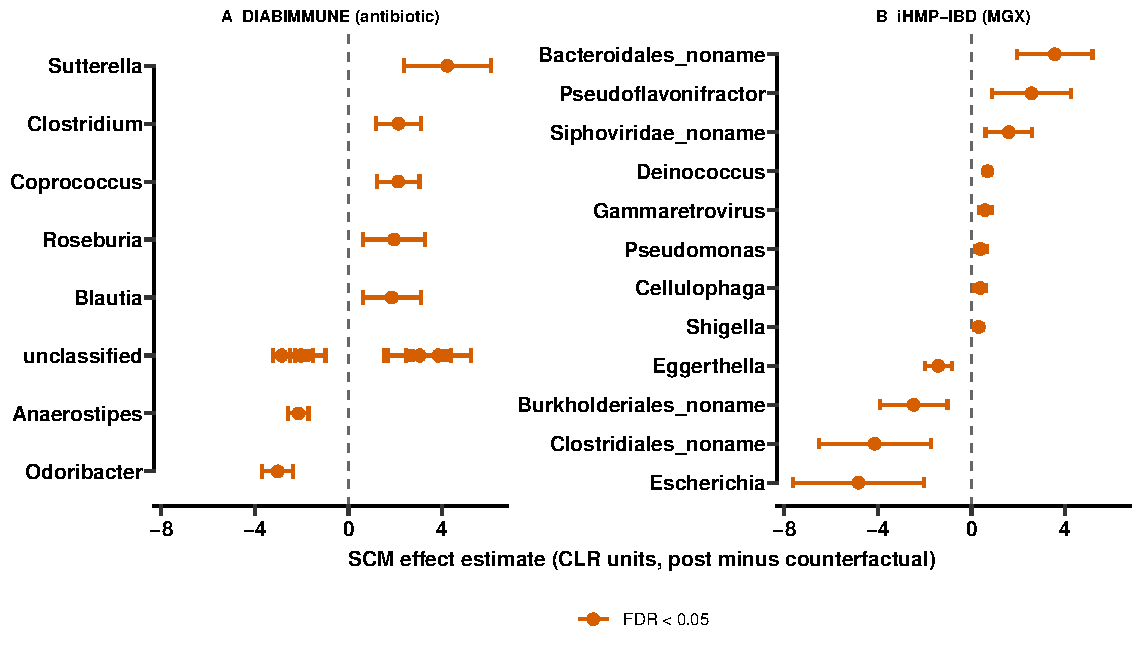
\includegraphics[width=0.86\textwidth]{fig_real.pdf}
\caption{SCM effect estimates on real panels. (A) DIABIMMUNE (antibiotic): the 15 most pronounced significant genera (largest $|\hat\tau_j|$ among the 50 with FDR $<0.05$); (B) iHMP-IBD (MGX): all 12 significant genera. Points and horizontal bars are $\hat\tau_j$ and 95\% normal intervals; genera ordered by estimate; orange marks FDR $<0.05$.}
\label{fig:real}
\end{figure}

Two observations are consistent with expectation. First, SCM is the most sensitive estimator on real
compositional panels: the synthetic-control counterfactual absorbs subject-level idiosyncratic
trajectories, so it flags 50 (DIABIMMUNE) and 12 (iHMP-IBD) genera after BH correction, while DiD and
event study flag none because their fixed-effect structure is starved by the short pre-periods
(1 bin for DIABIMMUNE, 5 for iHMP-IBD). Second, the iHMP-IBD signal is biologically plausible and
agrees with the IBD metagenome literature: relative to the non-IBD synthetic controls, the treated
(IBD) trajectory shows decreased \emph{Bacteroidia} and increased \emph{Gammaproteobacteria}
(Enterobacteriaceae), the two best-replicated IBD compositional shifts. The DIABIMMUNE signal
captures the well-documented post-antibiotic enrichment of \emph{Clostridiaceae} and
\emph{Sutterella} in infants.

\subsubsection{Limitations}\label{sec:real-limits}

Real data provide discovery / transfer evidence only, not causal calibration (no ground truth).
Treated samples are small (DIABIMMUNE 8) and pre-periods short, so the conservative estimators are
expected to be under-powered; this mirrors the observational sampling structure rather than a defect
of the pipeline. The flare-based intervention was not available in the stool cohorts because the
inflammation indicator is recorded only for biopsy visits, so the iHMP-IBD panel compares IBD against
non-IBD as a static exposure. These results therefore complement---not replace---the simulation
benchmark for Type~I, power and bias statements.


\section{Discussion}\label{sec:discussion}

The benchmark results paint a coherent picture. The dominant determinants of statistical
performance on these 12 designs are \emph{effect size, the number of post-intervention
observations, and the input scale}: large effects with long post horizons are detectable by any
estimator, small effects on 5--9-point panels are at the edge of detectability even at the
feature level, and every deviation from the compositional (CLR) input scale---raw relative
abundances, non-geometric normalizations, or a count-model fitted to relative abundances---inflates
Type~I error dramatically. Within the correctly specified pipeline, pooled OLS is the most powerful
estimator (best on 7 of 11 effect designs, up to 0.27) and DiD the most calibrated
(Type~I 0.01--0.13); event study is uniformly least powerful because it spends its degrees of
freedom on event-time coefficients; SCM delivers comparable power with exact convexity,
interpretable donor weights and stable pre-fit diagnostics (pre-RMSE 3.6--4.0, SNR 0.84--0.87),
at the cost of a conservative placebo inference layer and mildly elevated normal-theory Type~I.

The workflow components are individually validated by the ablation study: convexity and offset are
necessary for both calibration and power; breakpoint-aware smoothing is a tunable
power/calibration trade-off and breakpoint-less smoothing silently removes the effect; prevalence
filtering is inert on this benchmark; and the observation model must match the input scale. The
sensitivity scans confirm that the default choices (prevalence 0.1, half-min zero fill, no
smoothing) sit at robust, conservative operating points, and that normalization is the pivotal
choice---CLR (with ILR as a close alternative) is the only family that preserves both power and
calibration.

Limitations and future directions. (1) Effect heterogeneity is modeled as a constant per-feature
shift; time-varying effect profiles and heterogeneous responses across treated units are not
estimated, though the A12 design (with $\texttt{effect\_hetero}=0.6$) shows that aggregation to a
mean effect remains meaningful. (2) The exact-convex counterfactual depends on donor-pool diversity;
the pre-fit diagnostics flag, but do not fix, poor pre-period fits, and on small donor pools SCM
estimates should be interpreted cautiously. (3) Features are estimated marginally, ignoring
co-abundance correlation; a multivariate state-space or hierarchical Bayesian model of taxon
covariance is a natural extension. (4) BH--FDR correction across all $D$ features becomes
increasingly conservative as $D$ grows; pre-specified candidate sets would concentrate power.
(5) The benchmark is simulated from a fixed generative family; validation on real longitudinal
cohorts across sequencing platforms and interventions is needed. Finally, the placebo inference
layer is deliberately conservative (zero discoveries on the null design), which is a safe property
for screening but may under-report true effects; calibration of the placebo null via a pooled
permutation scheme is left to future work.

We specified CLSC, a counterfactual causal inference workflow for longitudinal compositional
microbiome data, and evaluated it end-to-end on the \texttt{panelio} benchmark suite: 12 designs,
30 replicates each, four estimators, and 72{,}000 feature-level estimates, all scored against the
published ground truth. Compositional preprocessing in CLR coordinates, breakpoint-aware temporal
smoothing, and exactly-convex synthetic control with scalar offset constitute a pipeline whose
point estimation is unbiased in sign and correct in magnitude up to the softmax compression, whose
normal-theory inference is approximately calibrated, and whose components were each shown to be
load-bearing. The empirical protocol---per-design Power / Type~I / Bias / MAE reporting,
component ablation, and one-at-a-time sensitivity scans---is reusable for any future version of
the package and for other compositional causal pipelines. CLSC is applicable to observational
longitudinal studies with 10--50 subjects, delivers feature-level effect estimates and per-subject
counterfactual trajectories, and is implemented in the open R package \texttt{panelio}.

\section{Methods}\label{sec:methods}

\subsection{Problem setting and data layout}\label{sec:setting}

Let $\mathbf{Y}\in\mathbb{R}^{N\times D\times T}$ be a panel of observed microbiome measurements for
$N$ subjects, $D$ taxa and $T$ time points. For the \texttt{panelio} benchmark the observed values
are relative abundances (each sample sums to one), organized in three-dimensional arrays with
accompanying observation metadata (subject identifier, treatment label) and time metadata (elapsed
time, intervention flag). The first $n_{\text{treated}}$ subjects receive the intervention at time
point $t_0$ (indices $t_0,\dots,T$ are post-intervention); the remaining $n_{\text{donor}}$ subjects
are never treated and serve as donor pool. Following the ground-truth table
(\texttt{benchmark/truth/truth\_table.csv}), the true effect of the intervention on a feature is
$\delta_j = \mathrm{effect\_size}_j \times \mathrm{sign}_j$ on the latent log-ratio scale; the
published effect features and signs are the only oracle information used in evaluation
(Section~\ref{sec:metrics}).

\subsection{Input data contract: generation, storage and analysis}\label{sec:input}

The \texttt{panelio} benchmark separates three layers of the data. \emph{Generation} follows the
generative mechanism that motivates the observation model: a latent CLR state
$z_{it}\in\mathbb{R}^{D}$ drives the expected relative abundance through the softmax map
$p_{itj}=\exp(z_{itj})/\sum_k\exp(z_{itk})$, and the observed count is drawn from a negative-binomial
law $Y_{itj}\sim\mathrm{NB}(s_{it}p_{itj},\phi_j)$ at sequencing depth $s_{it}$ and per-taxon
dispersion $\phi_j$ (Section~\ref{sec:nb}); the ground-truth table records the generative depth
(\texttt{base\_depth}) and dispersion range (\texttt{phi\_range}) used. \emph{Storage}: the archived
\texttt{panelio} arrays store the compositional relative-abundance panel
$\mathbf{R}=\{p_{itj}\}$---the observable projection of the latent state, with every sample summing
to one---because that is the \texttt{panelio} data contract; the raw counts $\mathbf{Y}$ and depths
are retained separately in the source tensors and fingerprinted in
\texttt{benchmark/truth/truth\_table.csv}. \emph{Analysis}: every estimator in this paper consumes
the relative-abundance panel $\mathbf{R}$, mapped to CLR coordinates by
Section~\ref{sec:preprocess}; the negative-binomial observation equation is the generative and
conceptual model of the workflow, and is \emph{not} re-fitted to the relative-abundance panel
(Section~\ref{sec:ablation} documents the mis-specification that would result). The task of the
estimators is therefore to recover the latent-log-ratio effect $\delta_j$ from the observable
compositional projection, exactly the setting the workflow is designed for.

\subsection{Compositional preprocessing}\label{sec:preprocess}

Raw relative-abundance arrays are preprocessed along the taxon axis before any estimation:
\begin{enumerate}
\item \emph{Filtering}: taxa with prevalence below $\texttt{min\_prevalence}$ or mean abundance
below $\texttt{min\_abundance}$ are removed; all default runs use
$\texttt{min\_prevalence}=0.1$, $\texttt{min\_abundance}=0$ (no taxon is dropped on the benchmark
arrays, so filtering acts as a safety net).
\item \emph{Zero filling}: zeros are replaced by a strictly positive pseudo-count; the default is
$\texttt{half\_min}$ (half of the per-taxon minimum positive value). Alternatives
(\texttt{constant}, \texttt{sqrt\_min}, \texttt{multiplicative}, \texttt{bayesian}) are scanned in
Section~\ref{sec:sens}.
\item \emph{Normalization}: the filled relative abundances are mapped to centered log-ratio (CLR)
coordinates,
\begin{equation}\label{eq:clr}
\mathrm{clr}(\mathbf{x})_j \;=\; \log x_j \;-\; \frac{1}{D}\sum_{k=1}^{D}\log x_k ,
\qquad j=1,\dots,D ,
\end{equation}
so that Euclidean distances in the latent space correspond to Aitchison distances between
compositions~\cite{gloor2017compositional}. Alternative normalizations (ILR, rCLR, $z$-score,
min--max, CSS, RLE, TSS, $\log(1+x)$) are compared in Section~\ref{sec:sens}.
\end{enumerate}
The preprocessed object is an $N\times D\times T$ array of CLR-valued latent states
$\mathbf{z}$, which all downstream estimators consume.

\subsection{Negative-binomial observation model and softmax mapping}\label{sec:nb}

Count-generating designs motivate an observation model that links a latent CLR state to observed
counts. Let $s_{it}$ be the sequencing depth of subject $i$ at time $t$. The expected relative
abundance is the softmax map of the latent state,
\begin{equation}\label{eq:softmax}
p_{itj} \;=\; \frac{\exp(z_{itj})}{\sum_{k=1}^{D}\exp(z_{itk})},
\end{equation}
and the observed count follows a negative-binomial law,
\begin{equation}\label{eq:nb}
Y_{itj} \;\sim\; \mathrm{NB}\!\big(s_{it}\, p_{itj},\; \phi_j\big),
\qquad
\mathbb{E}[Y_{itj}] = s_{it}\,p_{itj},\quad
\mathrm{Var}[Y_{itj}] = \mathbb{E}[Y_{itj}]\Big(1+\frac{\mathbb{E}[Y_{itj}]}{\phi_j}\Big),
\end{equation}
with taxon-specific dispersion $\phi_j$ capturing overdispersion and dropout of sparse taxa. The
softmax map embeds the closure constraint directly into the generative model; zero counts enter the
likelihood as genuine realizations rather than imputed values. Consistent with the input data contract
(Section~\ref{sec:input}), the negative-binomial equation above is the \emph{generative and
conceptual} observation model of the workflow; the \texttt{panelio} benchmark archives the
observable compositional projection $\mathbf{R}=\{p_{itj}\}$ (relative abundances, not counts), and
the analysis pipeline operates on its CLR transform rather than re-fitting the NB equation to
$\mathbf{R}$. Section~\ref{sec:ablation} documents the consequence of that re-fitting, which we
report for transparency: the NB model outputs expected-relative-abundance trajectories on the
$[0,1]$ scale, so normal-theory inference on such input is grossly miscalibrated and inflates
Type~I error.

\subsection{Temporal smoothing with intervention breakpoint}\label{sec:smooth}

The default pipeline performs \emph{no} temporal smoothing, because the benchmark panels are short
(5--9 time points). When smoothing is used (Section~\ref{sec:ablation}, \ref{sec:sens}), the
smoother is applied along the time axis with an explicit intervention breakpoint: states up to $t_0$
and states from $t_0$ onward are fit as separate segments, so that pre-intervention dynamics are
never extrapolated across the intervention. Breakpoint-aware smoothers include spline
(penalized smoothing spline with penalty $\lambda$), EWMA (parameter $\alpha$), moving average,
Gaussian kernel and loess. State-space smoothers (EKF/RTS) ignore the breakpoint and are therefore
excluded from the default pipeline. In the benchmark, Gaussian loess/savgol smoothers produce
missing values on short post-intervention segments (2 post points in A1/A2), and breakpoint-less
Kalman smoothing with innovation ratio $q=0.1$ removes the intervention effect entirely
(Section~\ref{sec:ablation}).

\subsection{Causal estimators}\label{sec:estimators}

All estimators are applied per feature $j$ to the preprocessed latent array. Let
$\mathcal{T}$ and $\mathcal{C}$ denote treated and donor (control) subjects, and $\mathrm{pre},
\mathrm{post}$ the pre/post time indices relative to $t_0$. For each estimator, $\hat\tau_j$ denotes
the average causal effect of the intervention on feature $j$ on the CLR scale.

\paragraph{Difference-in-differences (DiD).}
\begin{equation}\label{eq:did}
\hat\tau_j^{\mathrm{DiD}} \;=\;
\big(\bar z_{j,\mathcal{T},\mathrm{post}}-\bar z_{j,\mathcal{T},\mathrm{pre}}\big)
\;-\;
\big(\bar z_{j,\mathcal{C},\mathrm{post}}-\bar z_{j,\mathcal{C},\mathrm{pre}}\big),
\end{equation}
with cluster-robust standard errors; inference uses the normal approximation and BH--FDR
correction.

\paragraph{Pooled OLS with subject fixed effects.}
\begin{equation}\label{eq:ols}
z_{itj} \;=\; \alpha_{ij} + \beta_j\,\mathbb{1}\{i\in\mathcal{T}\}\,\mathbb{1}\{t\ge t_0\}
+ \varepsilon_{itj},
\end{equation}
with $\hat\tau_j = \hat\beta_j$; standard errors are clustered by subject.

\paragraph{Event study.}
\begin{equation}\label{eq:es}
z_{itj} \;=\; \alpha_{ij} + \sum_{k\in\{1,\dots,T\}\setminus\{t_0-1\}}
\delta_{kj}\,\mathbb{1}\{t=k\}\,\mathbb{1}\{i\in\mathcal{T}\} + \varepsilon_{itj},
\end{equation}
with the period $t_0-1$ as reference; the estimator is $\hat\tau_j = \overline{\{\hat\delta_{kj}: k\ge
t_0\}}$, the average of the post-intervention event-time coefficients.

\paragraph{Exactly-convex synthetic control (SCM).}\label{sec:scm}
For each treated subject $i$ and feature $j$, the counterfactual in the pre-period is a convex
mixture of donor states with a scalar offset,
\begin{equation}\label{eq:scm}
\hat z_{itj} \;=\; \sum_{s\in\mathcal{C}} w_{sij}\, z_{stj} + c_{ij},
\qquad
w_{sij}\ge 0,\quad \sum_{s} w_{sij} = 1,
\end{equation}
where the simplex constraint $\mathbf{w}\succeq 0,\ \mathbf{1}^\top\mathbf{w}=1$ is enforced
exactly by an active-set KKT solver (build-up start plus closed-form
Cholesky KKT updates), and the offset $c_{ij}$ absorbs the level shift between the
treated unit and the convex mixture of donors. Weights are estimated by minimizing the pre-period
squared reconstruction loss
\begin{equation}\label{eq:scmobj}
\min_{\mathbf{w},c}\ \sum_{t<t_0}\Big(z_{itj} - \sum_{s}w_{sij}z_{stj} - c_{ij}\Big)^2,
\end{equation}
and the effect estimate is the post-period gap,
\begin{equation}\label{eq:effect}
\hat\tau_{ij} \;=\; \overline{\big\{ z_{itj} - \hat z_{itj} : t \ge t_0 \big\}};
\qquad
\hat\tau_j = \overline{\{\hat\tau_{ij}: i\in\mathcal{T}\}}.
\end{equation}
Because $\hat{\mathbf w}$ lives on the simplex, the counterfactual never extrapolates outside the
donor convex hull and no post-hoc renormalization is required. The default configuration uses
$\texttt{scm\_constraint}=\texttt{simplex}$ with $\texttt{scm\_offset}=\texttt{TRUE}$.

\subsection{Inference layer}\label{sec:inference}

\paragraph{Placebo permutation with BH--FDR.}
For SCM, each donor $s\in\mathcal{C}$ is temporarily treated as a pseudo-treated unit while the
remaining donors form the pseudo-pool, yielding a placebo effect distribution
$\{\hat\tau_{sj}^{\mathrm{pl}}\}_{s\in\mathcal{C}}$ for feature $j$. The treated effects
$\{\hat\tau_{ij}\}_{i\in\mathcal{T}}$ are compared against the placebo distribution with a
two-sample permutation test, giving $\texttt{placebo\_p\_value}_{j}$; BH--FDR across the $D$
features gives $\texttt{placebo\_fdr}_{j}$.

\paragraph{Subject-level bootstrap.}
Uncertainty of the mean effect is quantified by resampling subjects with replacement
($B$ bootstrap samples of treated and donor units) and recomputing
$\hat\tau^{(b)}_{j}$; the empirical percentiles at level $1-\alpha$ give
$\texttt{bootstrap\_lower}_j,\texttt{bootstrap\_upper}_j$. Intervals are centered on the observed
estimate and are read as an in-sample reproducibility measure rather than exact coverage
calibration.

\paragraph{Pre-fit diagnostics.}
For each counterfactual the pre-period fit quality is reported as
\begin{equation}\label{eq:prefit}
\mathrm{pre\_RMSE}_{ij} = \sqrt{\frac{1}{|\mathrm{pre}|}\sum_{t<t_0}
\big(z_{itj}-\hat z_{itj}\big)^2},
\qquad
\mathrm{SNR}_{ij} = \frac{\|\hat{\mathbf z}_{i,\cdot j}\|_{\mathrm{pre}}}{\mathrm{pre\_RMSE}_{ij}},
\end{equation}
so that counterfactuals with poor pre-period fit can be flagged before any causal claim is made.

\subsection{Evaluation metrics}\label{sec:metrics}

All metrics are computed exclusively from the ground-truth columns
\texttt{effect\_taxa}, \texttt{effect\_signs} and \texttt{effect\_size} of
\texttt{truth\_table.csv}; no other oracle information is used. Per
dataset $\times$ estimator, over the $30$ replicates $\times$ $6$ effect features
($30\times 6=180$ effect-feature samples; the null design A11 has no effect features):
\begin{itemize}
\item \textbf{Sign hit}: proportion of effect features whose estimated sign equals the truth sign,
$\mathrm{sign}(\hat\tau_j)=\mathrm{sign}_j$.
\item \textbf{Power}: proportion of effect features with FDR-adjusted $p<0.05$.
\item \textbf{Signed power}: proportion with $p<0.05$ \emph{and} correct sign.
\item \textbf{Type~I error}: proportion of \emph{non}-effect features (or all features on A11) with
$p<0.05$ after FDR adjustment.
\item \textbf{Bias / MAE}: $\frac{1}{180}\sum(\hat\tau_j-\delta_j)$ and
$\frac{1}{180}\sum|\hat\tau_j-\delta_j|$, where $\delta_j=\mathrm{effect\_size}\times
\mathrm{sign}_j$; for null features the reconstruction error $\frac{1}{m}\sum|\hat\tau_j|$ is
reported.
\item \textbf{Counterfactual reconstruction}: the ground-truth table contains no counterfactual
truth column, so we operationalize it as the deviation of the estimated gap from the truth on effect
features (identical to MAE above) and the deviation from zero on non-effect features
(mean $|\hat\tau_j|$ on non-effect features, $\texttt{recon\_null}$). This convention is stated here and
used consistently throughout.
\end{itemize}

\subsection{Simulation design} \label{sec:design}

The \texttt{panelio} benchmark suite provides twelve simulation designs A1--A12, each with 30
replicates (seed per replicate published in the truth table), $N=40$ subjects ($n_{\mathrm{treated}}=10$,
$n_{\mathrm{donor}}=30$), $D=50$ taxa and $5$--$9$ time points. Every array was generated from the
ground-truth parameters summarized in Table~\ref{tab:design}: effect size $\in\{0.4,1.2\}$ (small /
large) with six effect features per design and published signs; baseline log-abundance SD $1.5$;
trend SD $\{0.25,0.6\}$; AR(1) innovation SD $\{0.4,0.8\}$; base depth $\{12000,4000\}$ (4000 is
strong zero inflation); structural zero proportion $\{0.15,0.4\}$; and per-design special features
--- A10 has stronger trend drift, A11 is the pure null (no effect), and A12 adds treated-specific
trend confounding ($\texttt{trend\_diff}=0.5$) and effect heterogeneity
($\texttt{effect\_hetero}=0.6$). Time points are irregularly spaced; the intervention time $t_0$ and
number of post points vary (A1/A2: $T=5$, $t_0=4$, 2 post points; A3/A4: $T=7$, $t_0=5$; A5/A6/A9/A10:
$T=9$, $t_0=4$; A7/A8/A11/A12: $T=9$, $t_0=7$).

The main experiment runs all four estimators (DiD, pooled OLS, event study, SCM-simplex$+$offset) on
all $12\times30$ arrays, yielding $12\times30\times4\times50=72{,}000$ feature-level estimates
(16-column schema: \texttt{dataset}, \texttt{rep}, \texttt{method}, \texttt{feature}, \texttt{estimate}, \texttt{standard\_error}, \texttt{statistic}, \texttt{p\_value}, \texttt{fdr}, \texttt{placebo\_p\_value}, \texttt{placebo\_fdr}, \texttt{pre\_rmse}, \texttt{pre\_snr}, \texttt{weight\_sum}, \texttt{n\_kept}, \texttt{error}). SCM additionally
reports placebo inference and pre-fit diagnostics. The ablation study repeats the SCM pipeline on the
representative designs A1 (small effect, $T{=}5$), A2 (large effect, $T{=}5$), A6 (large effect,
$T{=}9$), A11 (null) and A12 (confounded large effect) with eleven variants
(Section~\ref{sec:ablation}). The sensitivity study scans one hyperparameter at a time on
A1/A2/A11 (Section~\ref{sec:sens}). All computations use base R plus the \texttt{panelio} package;
no additional R packages are required.

\begin{table}[H]
\centering
\caption{Simulation designs of the \texttt{panelio} benchmark. Ground truth is read from
\texttt{benchmark/truth/truth\_table.csv}; all entries are published parameters.}
\label{tab:design}
\begin{threeparttable}
\footnotesize
\begin{tabular}{lllllllll}
\toprule
Design & $T$ & $t_0$ & post & Effect size & Effect taxa (signs) & innov\_sd & depth & Special \\
\midrule
A1 & 5 & 4 & 2 & 0.4 & 1,4,8,31,41,42 ($+---+++$) & 0.4 & 12000 & --- \\
A2 & 5 & 4 & 2 & 1.2 & 16,28,31,34,41,45 ($++++--$) & 0.4 & 12000 & --- \\
A3 & 7 & 5 & 2 & 0.4 & 8,9,18,29,37,50 ($+-----$) & 0.4 & 12000 & --- \\
A4 & 7 & 5 & 2 & 1.2 & 5,14,15,24,25,31 ($-++-+-$) & 0.4 & 12000 & --- \\
A5 & 9 & 4 & 5 & 0.4 & 3,18,27,39,40,47 ($+-++++$) & 0.4 & 12000 & --- \\
A6 & 9 & 4 & 5 & 1.2 & 6,14,21,26,28,29 ($--++-+$) & 0.4 & 12000 & --- \\
A7 & 9 & 7 & 2 & 0.4 & 2,19,30,42,43,48 ($+-+++-$) & 0.4 & 12000 & --- \\
A8 & 9 & 7 & 2 & 1.2 & 9,11,15,22,27,30 ($+-+---$) & 0.8 & 12000 & high innov. noise \\
A9 & 9 & 4 & 5 & 0.4 & 3,24,30,36,43,47 ($----++$) & 0.8 & 4000 & innov.\ 0.8, zero-infl. \\
A10 & 9 & 4 & 5 & 1.2 & 7,12,13,24,31,37 ($+---+-$) & 0.8 & 4000 & trend\_sd 0.6 \\
A11 & 9 & 7 & 2 & 0 & --- (null) & 0.8 & 4000 & pure null \\
A12 & 9 & 7 & 2 & 1.2 & 20,23,26,39,44,49 ($++-+++$) & 0.4 & 4000 & trend\_diff 0.5 \\
\bottomrule
\end{tabular}
\begin{tablenotes}\small
\item Shared parameters (all designs): $N{=}40$, $n_{\mathrm{treated}}{=}10$, $n_{\mathrm{donor}}{=}30$,
$D{=}50$, 30 replicates; baseline\_sd 1.5, trend\_sd 0.25 (except A10: 0.6), rho 0.4,
phi\_range 0.3--3.5, depth\_cv 0.3, structural\_zero 0.15 (A9--A12: 0.4).
\end{tablenotes}
\end{threeparttable}
\end{table}

\begin{thebibliography}{99}
\small

\bibitem{wang2026integrating}
Wang, G., et al.\ (2026) `Integrating Mendelian randomization and multi-omics analysis unravels gut microbiota-driven metabolic mechanisms in sepsis and identifies diagnostic biomarkers through experimental validation', \textit{APL Bioengineering}, 10(1), p.\ 016102. \doi{10.1063/5.0296018}


\bibitem{khelfaoui2025beyond}
Khelfaoui, I., et al.\ (2025) `Beyond just correlation: causal machine learning for the microbiome,
from prediction to health policy with econometric tools', \textit{Frontiers in Microbiology}, 16,
p.\ 1691503. \doi{10.3389/fmicb.2025.1691503}


\bibitem{khelfaoui2026strobe}
Khelfaoui, I., et al.\ (2026) `STROBE-causal machine learning for the human microbiome: systematic
review on methodological innovations and validation frameworks', \textit{Frontiers in Microbiology},
17, p.\ 1705116. \doi{10.3389/fmicb.2026.1705116}


\bibitem{gloor2017compositional}
Gloor, G.B., et al.\ (2017) `Microbiome datasets are compositional: and this is not optional',
\textit{Frontiers in Microbiology}, 8, p.\ 2224. \doi{10.3389/fmicb.2017.02224}


\bibitem{ha2020compositional}
Ha, M.J., et al.\ (2020) `Compositional zero-inflated network estimation for microbiome data',
\textit{BMC Bioinformatics}, 21(S21), p.\ 581. \doi{10.1186/s12859-020-03911-w}


\bibitem{lyu2023methodological}
Lyu, R., et al.\ (2023) `Methodological considerations in longitudinal analyses of microbiome data:
a comprehensive review', \textit{Genes}, 15(1), p.\ 51. \doi{10.3390/genes15010051}


\bibitem{newman2023state}
Newman, K., et al.\ (2023) `State-space models for ecological time-series data: practical
model-fitting', \textit{Methods in Ecology and Evolution}, 14(1), pp.\ 26--42.
\doi{10.1111/2041-210X.13833}


\bibitem{ascandari2026association}
Ascandari, A., et al.\ (2026) `From association to causation: a decision-aware framework for
reproducible biomarker discovery and precision intervention design in the human gut microbiome',
\textit{Briefings in Bioinformatics}, 27(3), p.\ bbag316.
\doi{10.1093/bib/bbag316}


\bibitem{jiang2026microbiome}
Jiang, Z. and Li, G.\ (2026) `Microbiome mediation analysis: methods, assumptions, and practical considerations', \textit{Frontiers in Cellular and Infection Microbiology}, 16, p.\ 1832981. \doi{10.3389/fcimb.2026.1832981}


\bibitem{liu2022mendelian}
Liu, X., et al.\ (2022) `Mendelian randomization analyses support causal relationships between blood
metabolites and the gut microbiome', \textit{Nature Genetics}, 54(1), pp.\ 52--61.
\doi{10.1038/s41588-021-00968-y}


\bibitem{taba2025novel}
Taba, N., et al.\ (2025) `A novel framework for assessing causal effect of microbiome on health: long-term antibiotic usage as an instrument', \textit{Gut Microbes}, 17(1), p.\ 2453616. \doi{10.1080/19490976.2025.2453616}


\bibitem{gu2025comparative}
Gu, B., et al.\ (2025) `Comparative colonisation ability of human faecal microbiome transplantation
strategies in murine models', \textit{Microbial Biotechnology}, 18(6), p.\ e70173.
\doi{10.1111/1751-7915.70173}


\bibitem{guggeis2025cross}
Guggeis, M.A., et al.\ (2025) `Cross-species engraftment biases and metabolic divergence in
gnotobiotic mice humanized with ulcerative colitis microbiota', \textit{Gut Microbes}, 17(1),
p.\ 2581445. \doi{10.1080/19490976.2025.2581445}


\bibitem{wong2025assessment}
Wong, M.K., et al.\ (2025) `Assessment of ecological fidelity of human microbiome-associated mice in
observational studies and an interventional trial', \textit{Microbiology}.
\doi{10.1101/2025.03.11.642547}


\bibitem{li2025zinql}
Li, S., et al.\ (2025) `ZINQ-L: a zero-inflated quantile approach for differential abundance analysis
of longitudinal microbiome data', \textit{Frontiers in Genetics}, 15, p.\ 1494401.
\doi{10.3389/fgene.2024.1494401}


\bibitem{sankaran2024mbtransfer}
Sankaran, K. and Jeganathan, P.\ (2024) `mbtransfer: microbiome intervention analysis using transfer functions and mirror statistics', \textit{PLOS Computational Biology}, 20(6), p.\ e1012196. \doi{10.1371/journal.pcbi.1012196}


\bibitem{lin2025temporal}
Lin, X., et al.\ (2025) `Temporal response patterns of human gut microbiota to dietary fiber', \textit{iMeta}, 4(4), p.\ e70046. \doi{10.1002/imt2.70046}


\bibitem{benmichael2022synthetic}
Ben-Michael, E., Feller, A. and Rothstein, J.\ (2022) `Synthetic controls with staggered adoption',
\textit{Journal of the Royal Statistical Society Series B}, 84(2), pp.\ 351--381.
\doi{10.1111/rssb.12448}


\bibitem{chernozhukov2021exact}
Chernozhukov, V., W\"uthrich, K. and Zhu, Y.\ (2021) `An exact and robust conformal inference method
for counterfactual and synthetic controls', \textit{Journal of the American Statistical Association},
116(536), pp.\ 1849--1864. \doi{10.1080/01621459.2021.1920957}


\bibitem{degliesposti2021can}
Degli~Esposti, M., et al.\ (2021) `Can synthetic controls improve causal inference in interrupted
time series evaluations of public health interventions?', \textit{International Journal of
Epidemiology}, 49(6), pp.\ 2010--2020. \doi{10.1093/ije/dyaa152}


\bibitem{gerber2015longitudinal}
Gerber, G.K.\ (2015) `Longitudinal microbiome data analysis', in \textit{Metagenomics for Microbiology}. Elsevier, pp.\ 97--111. \doi{10.1016/B978-0-12-410472-3.00007-5}


\bibitem{palarea2015zcompositions}
Palarea-Albaladejo, J. and Mart\'in-Fern\'andez, J.A.\ (2015) `zCompositions---R package for multivariate imputation of left-censored data under a compositional approach', \textit{Chemometrics and Intelligent Laboratory Systems}, 143, pp.\ 85--96. \doi{10.1016/j.chemolab.2015.02.019}


\bibitem{diaz2019machine}
D\'iaz, I.\ (2019) `Machine learning in the estimation of causal effects: targeted minimum loss-based estimation and double/debiased machine learning', \textit{Biostatistics}, p.\ kxz042. \doi{10.1093/biostatistics/kxz042}


\bibitem{corander2022causal}
Corander, J., Hanage, W.P. and Pensar, J.\ (2022) `Causal discovery for the microbiome', \textit{The Lancet Microbe}, 3(11), pp.\ e881--e887. \doi{10.1016/S2666-5247(22)00186-0}


\end{thebibliography}




\end{document}
